\appendix

\section{Appendix} 

\subsection{Neural Neural Textures: More Details}

	In Section \ref{sec:neural_tex}, we mentioned that neural neural textures learn better than raster neural textures. 
	TRITON can be ablated to use raster textures. Let's call this version ``Raster TRITON''. 
	Raster TRITON is extremely sensitive to the resolution of its neural texture, and can be numerically unstable if that resolution is too high.
	In comparison, regular TRITON's neural neural textures do not have a specific resolution: they are continuously defined over the UV domain using Fourier feature networks.

	\begin{figure}[H]
		\begin{center}
			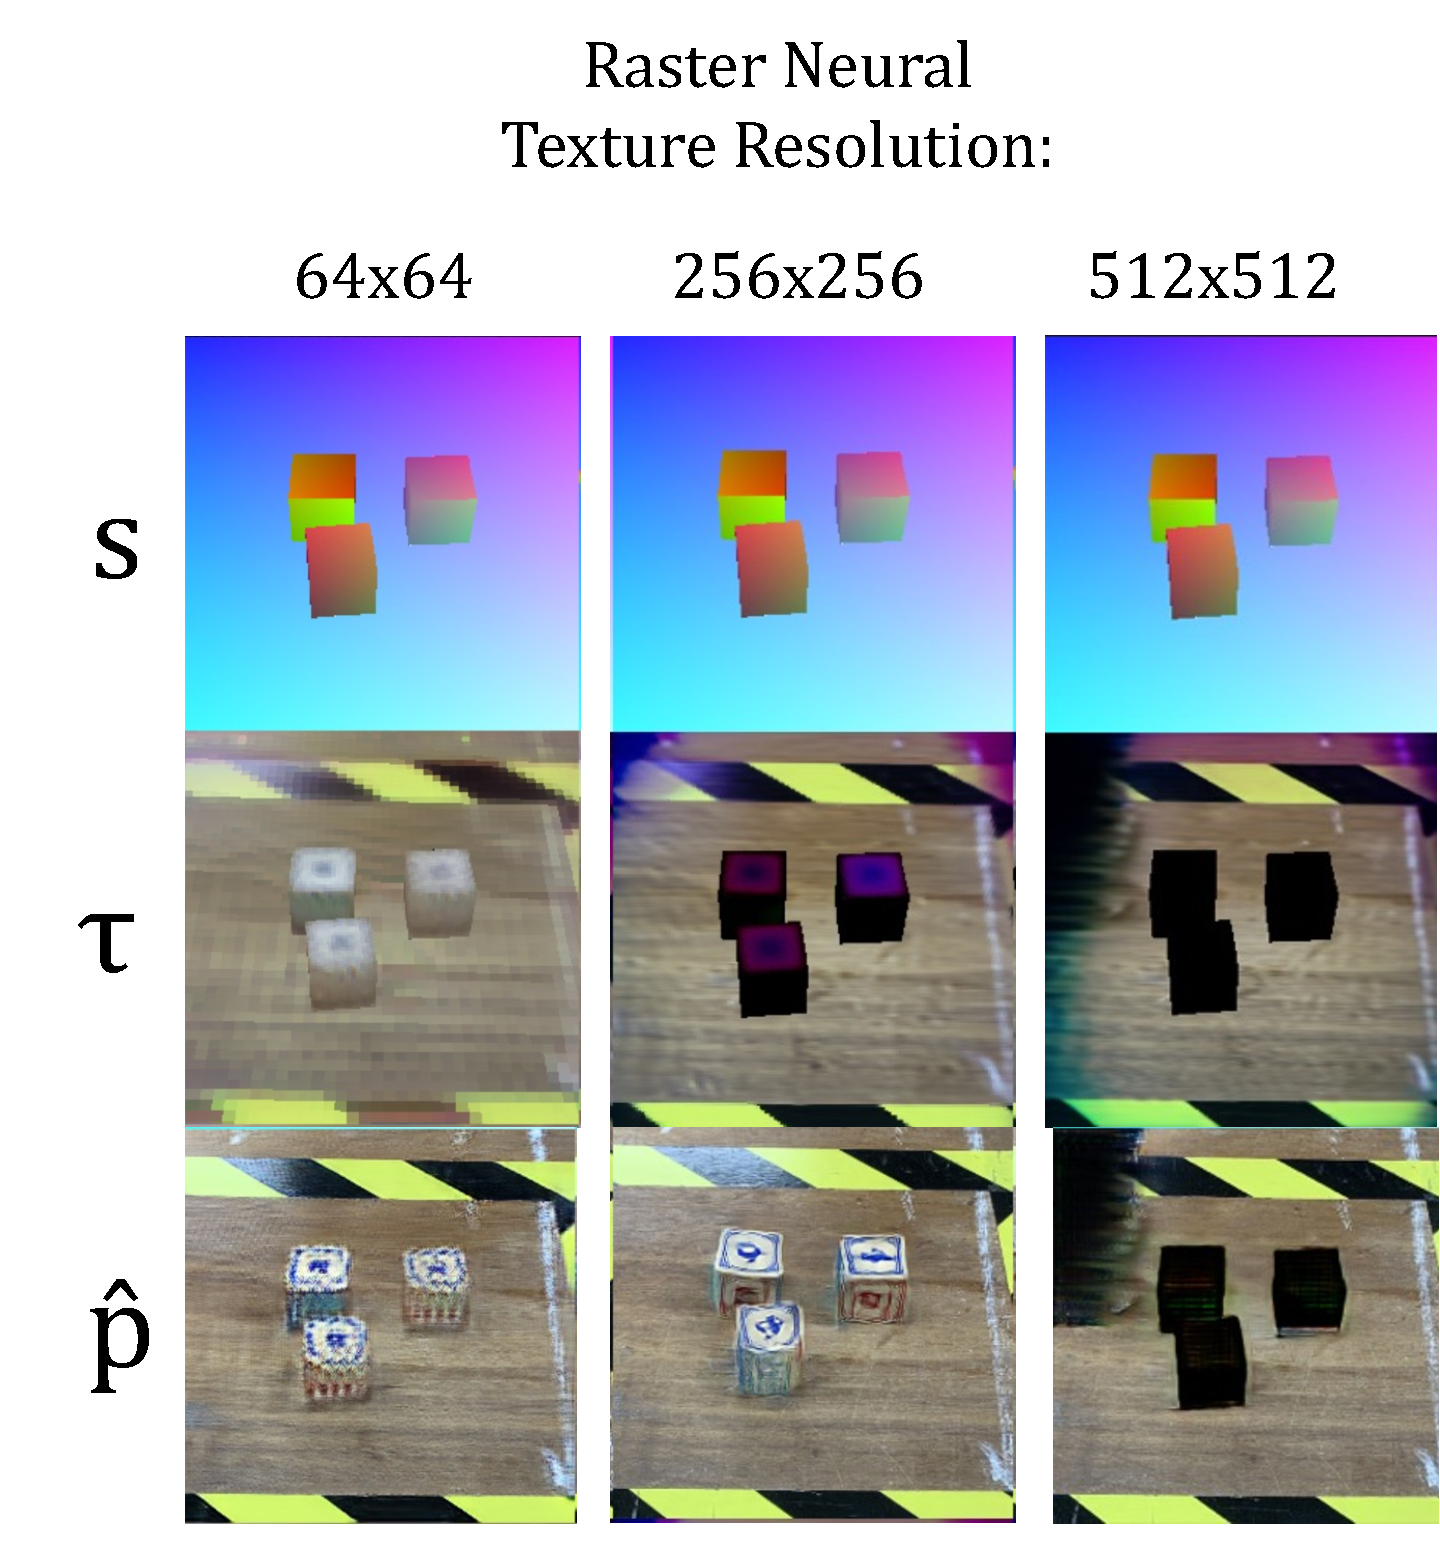
\includegraphics[width=400pt]{../images/raster_texture_resolution_comparisons.pdf}
		\end{center}
		\caption{
			The resolution of the raster neural texture seriously impacts performance in ``Raster TRITON''. Each column has a different neural texture resolution.
			The neural texture only looks like the translation when the resolution is low.
		}
		\label{fig:raster_texture_resolution_comparisons}
	\end{figure}

	In this paragraph we offer possible explanations for these observations.
	With raster-based textures, only the side of an object that currently is seen in a view is allowed to change during each update, because the gradient can not be propagated into pixels which are not seen.
	If this means changing overall brightness of an object for example, the brightness of that object can not be changed over the entire object until every side has been seen - which will not happen in a single iteration, since the batch size is limited.

	In addition to not propagating the gradient to unseen sides of objects, it also can not propagate to texels in-between the UVL values seen in a scene image.
	When the raster neural texture is too large, aliasing effects occur: if you have a raster texture with very high resolution, the loss gradient is less likely to be passed to a given texel because the chance that a given UV value in a scene will be rounded to that pixel's coordinates is very small.
	In practice, this makes large raster neural textures unstable and limits us to using small amounts of detail.
	With neural neural textures, this aliasing problem is mostly mitigated, because when a certain texture receives a gradient at particular UV coordinates, the areas of the texture between those coordinates are also changed.

\subsection{Unprojection Consistency Loss: More Details}

	Here, we give more details about unprojection consistency loss $\lUC$.

	The exact equation for $\lUC$ is as follows:
	to formally define $\lUC$ we define unprojections $\unprojection^{1...N,1...L}$ and mean unprojections (aka recovered textures) $\bar{\unprojection}^{1...L}$ 
	with each $\unprojection^{n,i}\in\real^{3\times128\times128}$:
	%Jinghyan's Version (uses expectation)
	% \begin{equation}
	% 	\unprojection_{U,V}^{n,i}=\expectation\ph_{x,y}^n 
	% 	\eqand \bar{\unprojection}^i_{u,v}   =   
	% 		\frac{1}{N} \lsum_n\unprojection^{n,i}_{u,v} 
	% 	\eqand 
	% 	%\lUC=\frac{\lsum_{i,U,V}
	% 	%\sqrt[]{\frac{1}{N}\lsum_n\left(\bar{\unprojection}^i_{u,v}-\unprojection^{i,n}_{U,V}\right)^2}}
	% 	%{128\cdot128\cdot L}
	% 	\lUC=\mathbb{E}\left[
	% 	\sqrt[]{\frac{1}{N}\lsum_n\left(\bar{\unprojection}^i_{u,v}-\unprojection^{i,n}_{U,V}\right)^2} \right]
	% \end{equation}
	%
	%
	%Unabbreviated: Not Jinguan's version; 
	\begin{multline}
		\unprojection_{c,U,V}^{n,i}=\expectation\ph_{c,x,y}^n 
		\eqand \bar{\unprojection}^i_{c,u,v}   =   
			\frac{1}{N} \lsum_{n=1}^N\unprojection^{n,i}_{c,u,v} 
		\eqand \\
		\lUC=\frac{\lsum_{i=1}^L\lsum_{c=1}^3\lsum_{U=1}^{128}\lsum_{V=1}^{128}
		\sqrt[]{\frac{1}{N}\lsum_{n=1}^N\left(\bar{\unprojection}^i_{c,u,v}-\unprojection^{i,n}_{c,U,V}\right)^2}}
		{3\cdot128\cdot128\cdot L}
	\end{multline}
	where $U=\lfloor128u\rfloor$ and $V=\lfloor128v\rfloor$ and $i=I(l)$ with
	%  $(u,v,l)=s^n_{1...3,x,y}$
	$u=s^n_{1,x,y}$, $v=s^n_{2,x,y}$, $l=s^n_{3,x,y}$
	for all 
	$n \in \{1...N\}$ , 
	$i \in \{1...L\}$ , 
	$x \in \{1...W\}$ , 
	$y \in \{1...H\}$ , 
	$U \in \{1...128\}$ , 
	$V \in \{1...128\}$.

	\bigskip
	
	The hyperparameter 128 we described in Section \ref{sec:unprojection_consistency_loss} refers to the resolution of the unprojections used to calculate $\lUC$.
	In Figure \ref{fig:unprojection_resolution_comparison} we see that if we were to set it higher, the gradient wouldn't affect the neural texture as densely.

	\begin{figure}[H]
		\begin{center}
			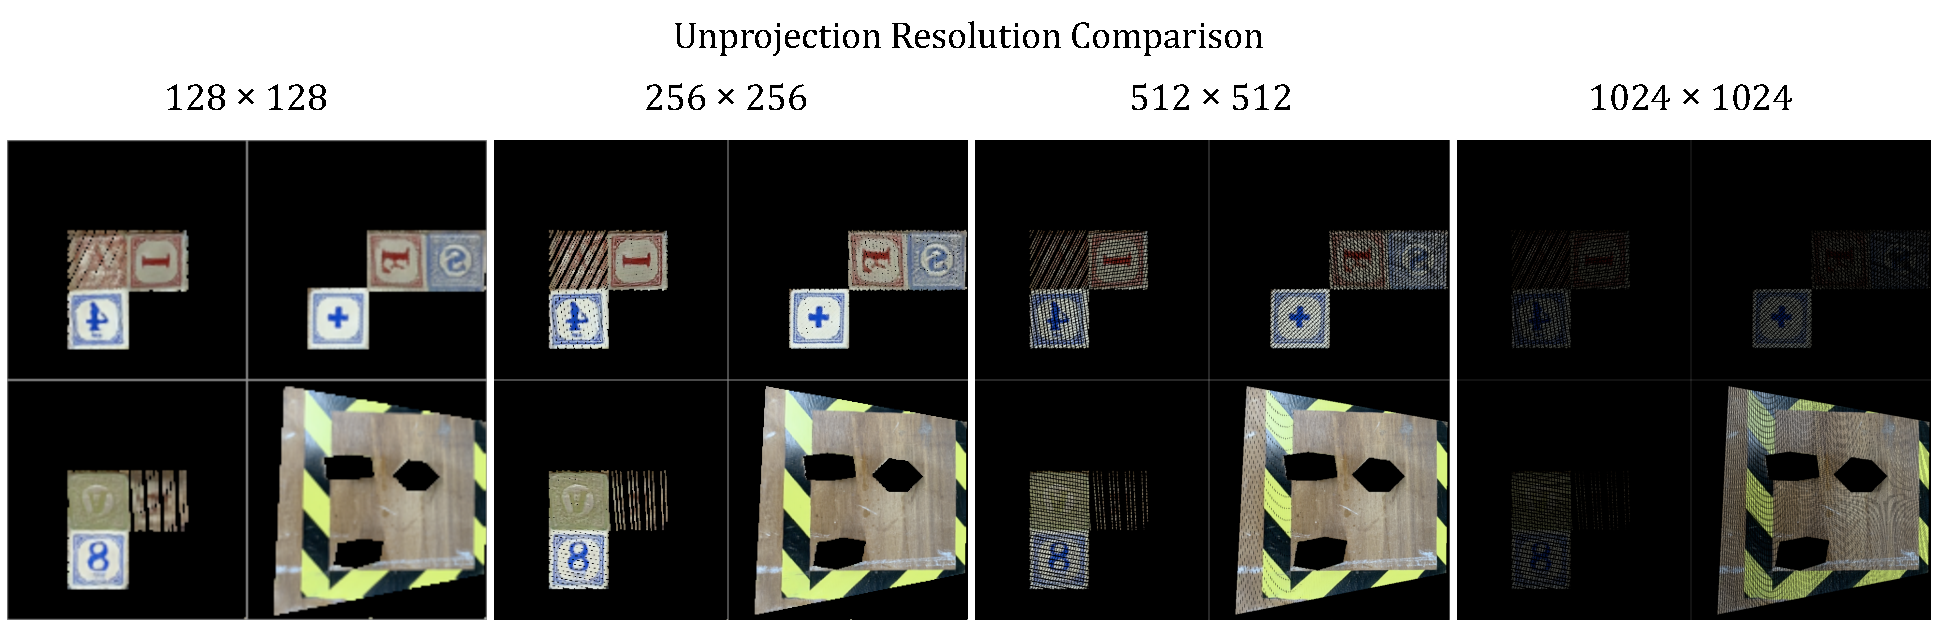
\includegraphics[width=400pt]{../images/unprojection_resolution_comparison.pdf}
		\end{center}
		\caption{
			Here, we unproject a single fake photo $\ph^i$. The resolution of the unprojection matters for unprojection consistency loss. The larger it is, the more precise the alignment will be but the less likely a given UV value is to be assigned a loss greater than 0, creating numerical instability and slowing down learning. 
			When the unprojection resolution is too high, only a few areas of the neural texture will receive a gradient during backpropogation. In practice we use the resolution $128\times128$.
		}
		\label{fig:unprojection_resolution_comparison}
	\end{figure}

\subsection{Training Procedures}

	In this section we detail the training procedures used to create results in Section \ref{sec:results} from Triton, CycleGAN, CUT,
		TRITON w/o $\lUC,\lTR$ (aka TRITON with neither unprojection consistency loss nor texture reality loss), and
		TRITON w/o $\psi, \lUC,\lTR$ (aka TRITON without textures, and therefore also without unprojection consistency loss or texture reality loss).

	\subsubsection{TRITON}
	\label{par:triton}
	We train TRITON for 200,000 iterations on all datasets. This takes about 36-48 hours on an NVIDIA RTX A5000. 
	The dimension of each input scene is defined by hyperparameter height $H$; the width is scaled to match the aspect ratio of the original input.
	To avoid running out of video memory, we randomly crop each input to a $256\times256$ subset and run TRITON on that cropped input.
	We use batch size 5 during training.
	
	We found that the best way to train TRITON is to start with smaller $H$ values and progressively increase that value during training.
	For the first 50,000 iterations we use $H=320$, then for the next 50,000 iterations $H=420$, then for the last 100,000 iterations $H=\text{(the height of the original input scene)}$.

	Like in \cite{surgical_video_translation}, we use three Adam optimizers: two for the translation module's encoders and decoders, and another for the neural texture.
	For the translation module's optimizers, we use learning rate $\num{1e-4}$, and for the neural neural texture we use learning rate $\num{1e-3}$. 
	Every 100,000 iterations all learning rates are halved.

	During evaluation, we render the neural neural texture onto a raster grid of pixels. Because the neural neural texture has a 2d manifold, it can be closely approximated by an RGB image. Using this method lets us avoid evlauating $\psi$'s fourier feature network on every frame by using a raster image as a lookup table. This decreases video memory usage and speeds up calulations during inference.

	\subsubsection{TRITON w/o $\lUC,\lTR$}
	\label{par:triton_without_luc}
	This ablation is also known as ``Texture-Only'' TRITON, because it has a learnable texture $\psi$ but no consistency losses.
	Its trained the same way that we train TRITON normally as discussed above in \ref{par:triton}, except the surface consistency losses $\lUC$ and $\lTR$ are omitted.
	Effectively, it performs better than MUNIT-like TRITON (aka TRITON w/o $\psi, \lUC,\lTR$, discussed in \ref{par:munit_triton})
	% It still has a learnable texture $\psi$ though, which is allowed to change however it likes.

	\subsubsection{TRITON w/o $\psi, \lUC,\lTR$}
	\label{par:munit_triton}
	This ablation is very similar to MUNIT, as TRITON is based on MUNIT and this ablation has neither learnable texture nor consistency losses.
	Like in subsection \ref{par:triton_without_luc}, this ablation shares the same training procedures as TRITON.

	\subsubsection{CycleGAN}
	\label{par:cyclegan}
	We use the original implementation of CycleGAN, and stick to the reccomended 200 epochs, as it tends to overfit if you go further. 
	For our tests, we run CycleGAN on multiple different scales of the input scenes, with input sizes $286\times286$ (CycleGAN's default), $320\times320$, $420\times420$ and $512\times512$. 
	After translation, we stretch the image into the input's aspect ratio.
	We also set $\lambda_{identity}=0$, meaning we disable the identity loss.
	The reported results are the calculated using the best results among these resolutions.
	This dramatically improves CycleGAN's performance when translating UVL scenes to photographs, as this loss was built with the assumption that some parts of the input should not be changed during translation (which is not true in our case).
	
	\subsubsection{CUT}
	\label{par:cut}
	We use the original implementation of CUT, and stick to the recommended 400 epochs, as it tends to overfit if you go further. 
	Like with CycleGAN in \ref{par:cyclegan}, we run CUT on multiple different resolutions of the input scenes, with input sizes $286\times286$ (CUT's default), $320\times320$, $420\times420$ and $512\times512$. 
	After translation, we stretch the image into the input's aspect ratio.
	The reported results are the calculated using the best results among these resolutions.

\subsection{More Results}

	\subsubsection{Unprojection Comparisons}

		In this section we expand on the results in Subsection \ref{sec:datasetsresults} by showing the mean unprojection (aka recovered texture) for different image translation algorithms. With the 14 UVL images and corresponding fake photos (or photos) as calculated in \ref{sec:datasetsresults}, we average their unprojections.
		If a translation algorithm is consistent, these unprojections should align well and the average $bar{\omega}$ should not be blurry.

		\begin{figure}[H]
			\begin{center}
				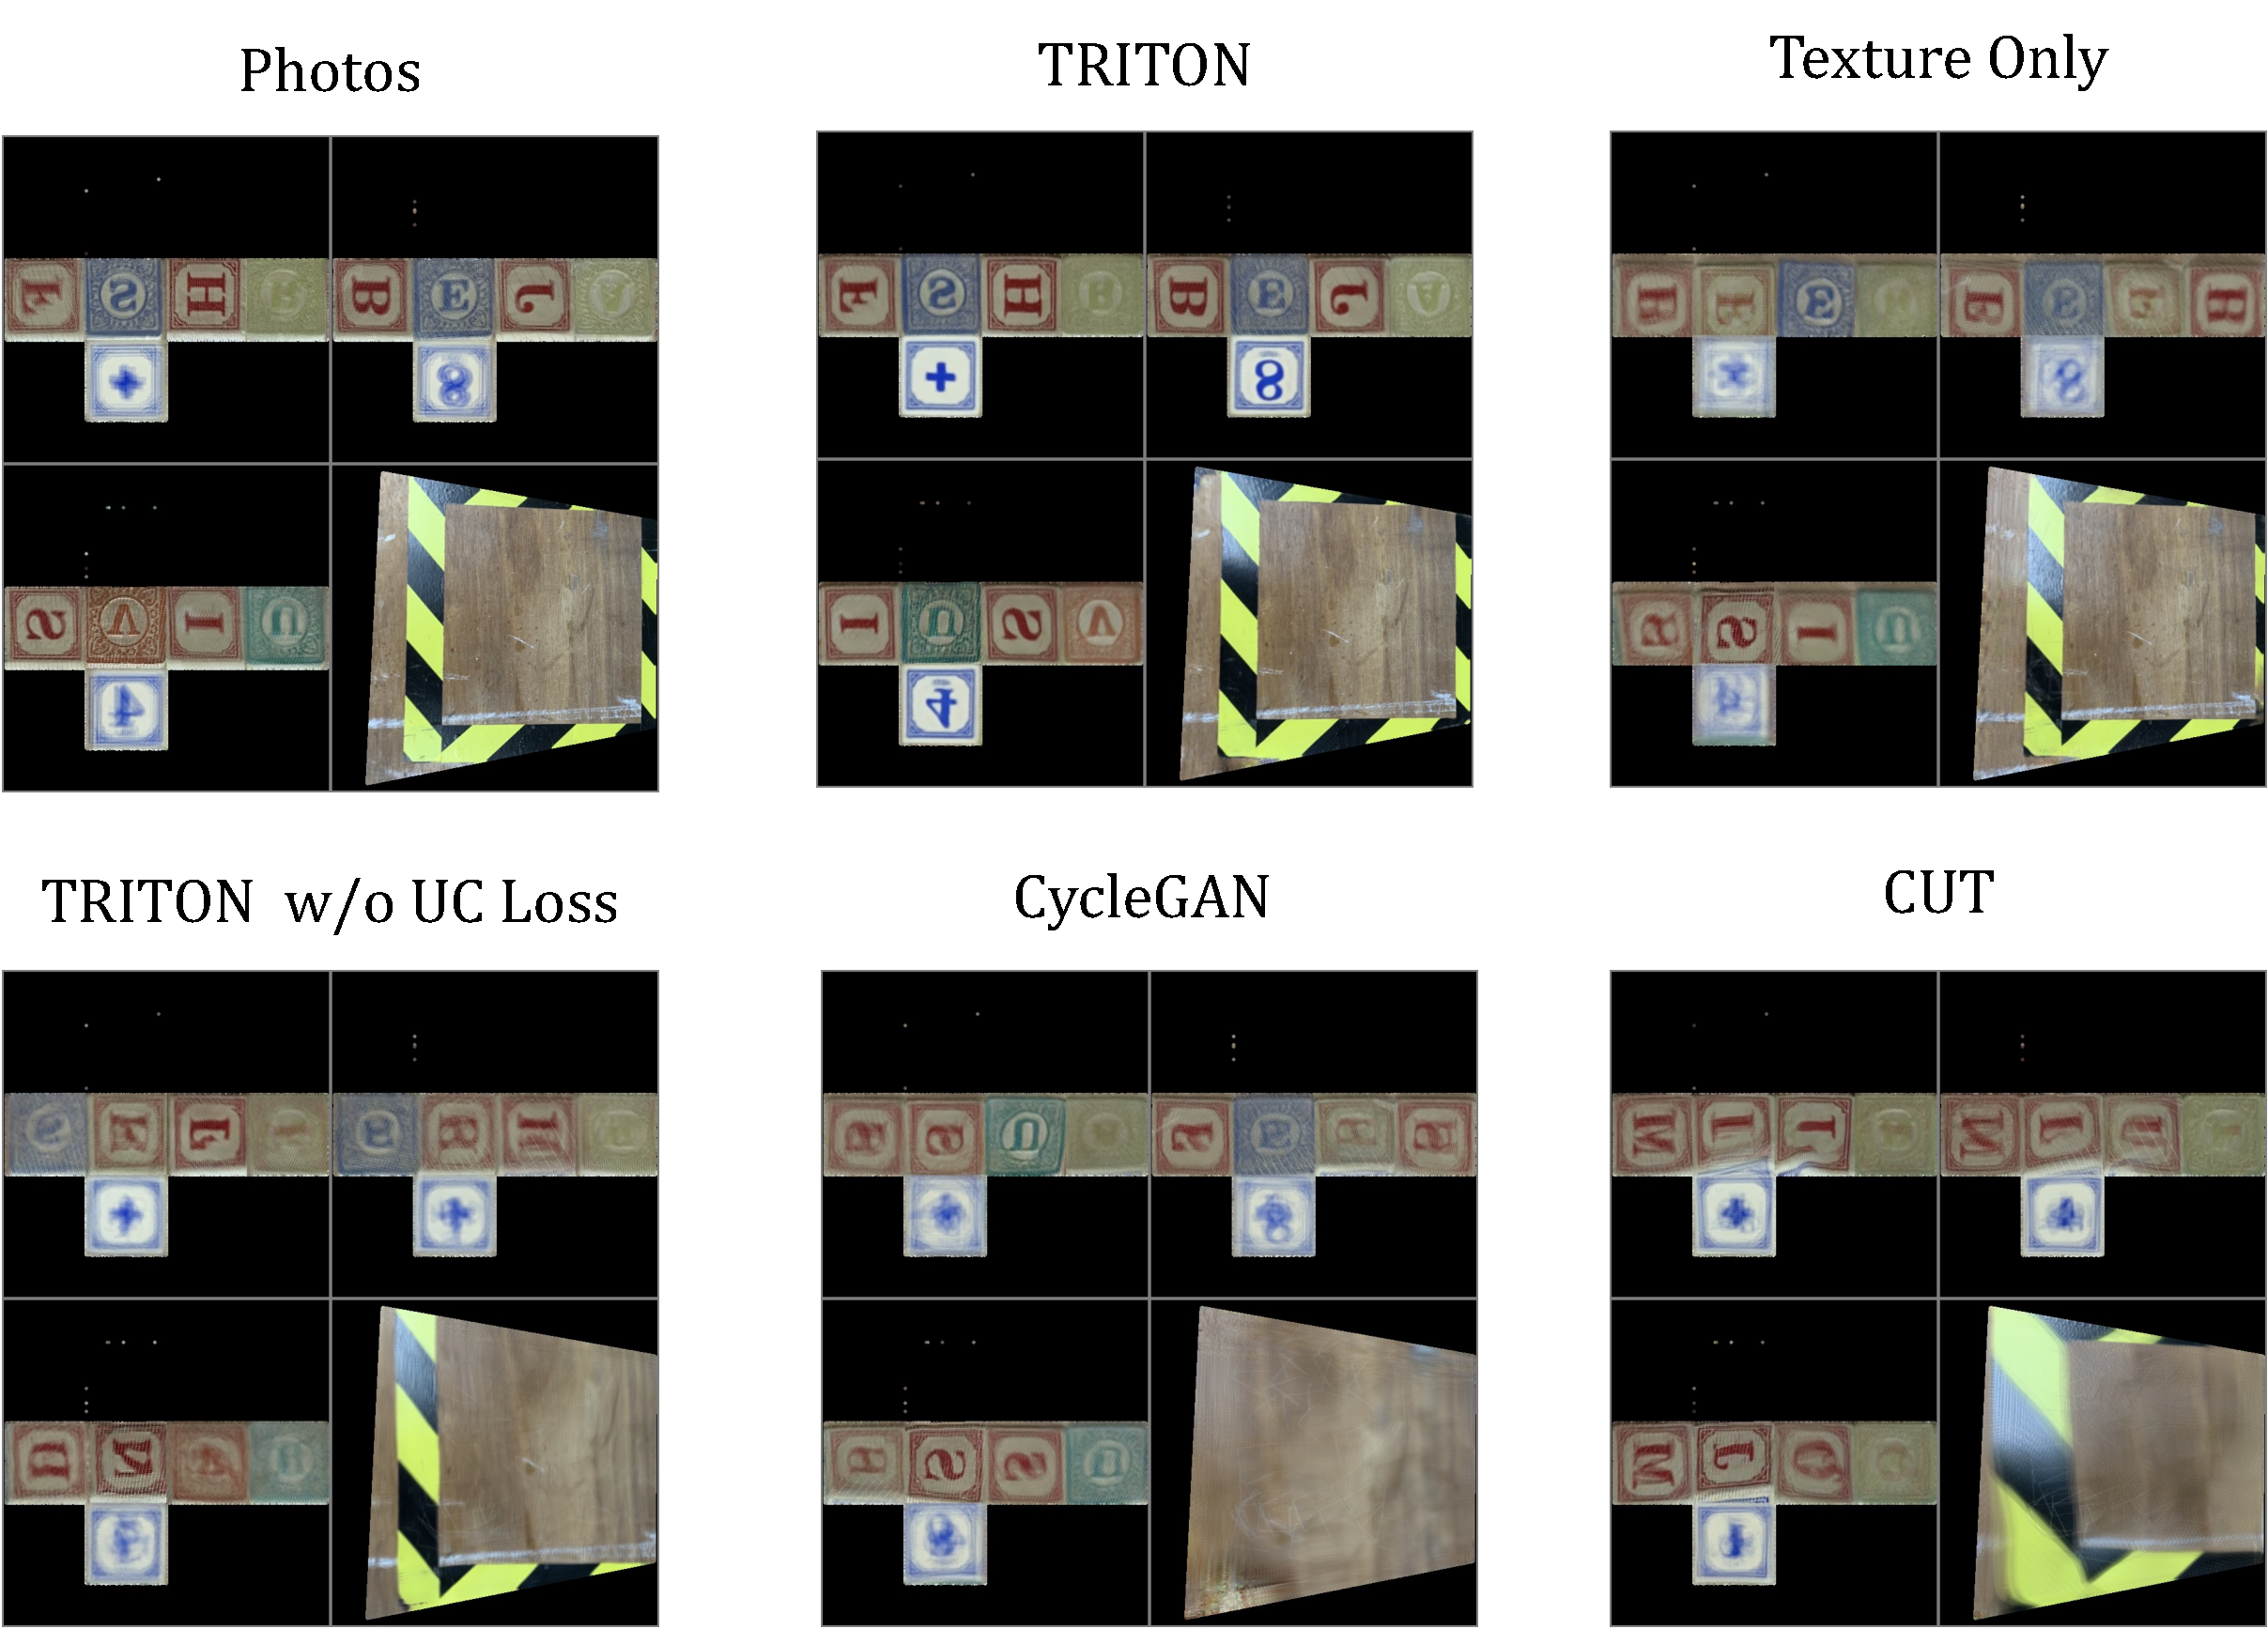
\includegraphics[width=400pt]{../images/unprojection_comparisons.pdf}
			\end{center}
			\caption{
				In this figure, we compare the recovered textures $\bar{\omega}$ (aka mean unprojections) of the 14 labeled images between different algorithms, and compare it to a ground truth. In this diagram, we align all the unprojections to make them easier to compare. Note how TRITON is more crisp and matches the unprojected photographs better than the other algorithms, which are blurrier and have the wrong colors and letters on each side of the alphabet blocks. CycleGAN and CUT for example incorrectly duplicate letters between alphabet blocks.
			}
			\label{fig:unprojection_resolution_comparison}
		\end{figure}

\pagebreak
	\subsubsection{Videos}

		In this section we have links to animations that help demonstrate various aspects of TRITON.
		If you are viewing this document on a computer, click a thumbnail to view the video.

		% https://youtu.be/fuTSta_M6NQ
	

		\begin{figure}[H]
			\begin{center}
			\href{https://youtu.be/kecK_cJgLT8}{
					\includegraphics[width=300pt]{../images/robot_arm_animation_thumbnail.png}
					}
				\end{center}
			\caption{
				This animation shows a side-by-side comparison of different camera viewpoints of the results discussed in Section \ref{sec:robotarm_results}, as well as the inputs, ground truth video, TRITON and TRITON ablation videos.
				Url: \href{https://youtu.be/kecK_cJgLT8}{youtu.be/kecK\_cJgLT8}
			}
			\label{fig:robotarm_anim}
		\end{figure}


		\begin{figure}[H]
			\begin{center}
			\href{https://youtu.be/0t0xiVS_8D0}{
					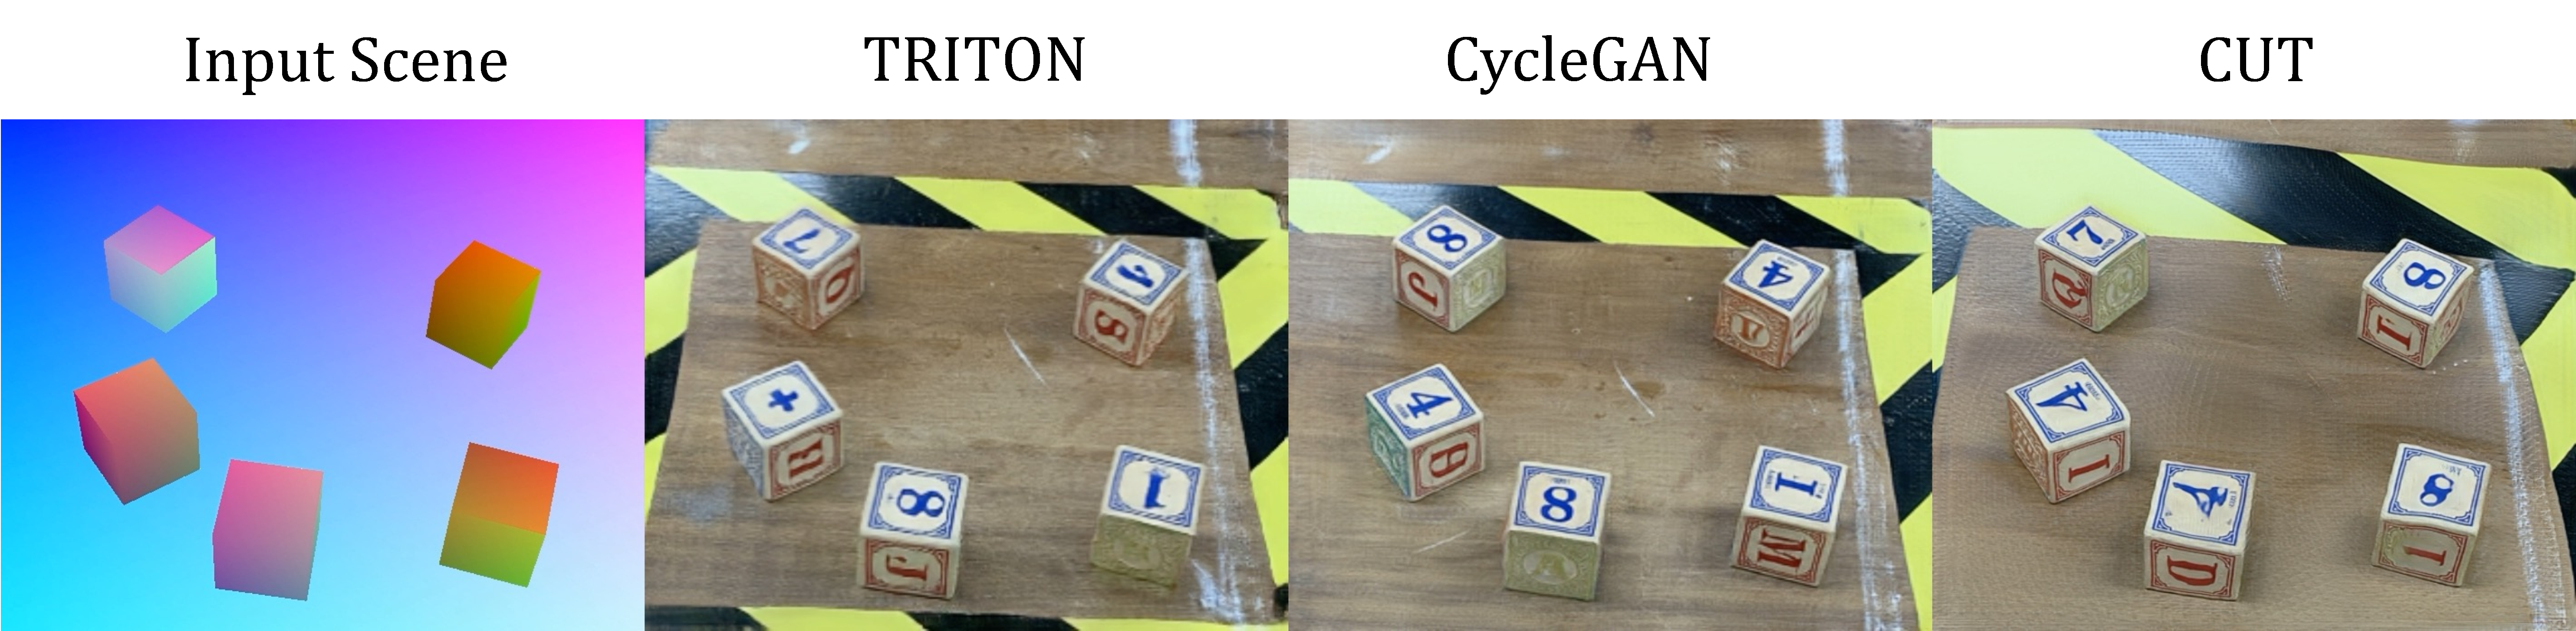
\includegraphics[width=300pt]{../images/algo_comparison_thumbnail.pdf}
					}
				\end{center}
			\caption{
				This animation shows an animation of various algorithms on a dataset with 5 alphabet blocks moving around. 
				When watching, note how the numbers on the top of the cubes in both CycleGAN and CUT change over time, while with TRITON they stay the same.
				Url: \href{https://youtu.be/0t0xiVS_8D0}{youtu.be/0t0xiVS\_8D0}
			}
			\label{fig:algocomparisonvideo}
		\end{figure}



		\begin{figure}[H]
			\begin{center}
			\href{https://youtu.be/0t0xiVS_8D0}{
					\includegraphics[width=300pt]{../images/ThreeDatasets.png}
					}
				\end{center}
			\caption{
				This video shows the results of TRITON applied on three of the datasets shown in Figure \ref{fig:first_diagram}.
				The top row shows the input scenes $s$, and the bottom row shows the fake photographs $\ph$.
				Url: \href{https://youtu.be/0t0xiVS_8D0}{youtu.be/0t0xiVS\_8D0}
			}
			\label{fig:algocomparisonvideo}
		\end{figure}



	

	



